\documentclass[sigchi-a, authorversion]{acmart}
\usepackage{booktabs} % For formal tables
\usepackage{ccicons}  % For Creative Commons citation icons
\usepackage{todonotes}

% Copyright
%\setcopyright{none}
%\setcopyright{acmcopyright}
\setcopyright{acmlicensed}
%\setcopyright{rightsretained}
%\setcopyright{usgov}
%\setcopyright{usgovmixed}
%\setcopyright{cagov}
%\setcopyright{cagovmixed}


% DOI
\acmDOI{10.475/123_4}

% ISBN
\acmISBN{123-4567-24-567/08/06}

%Conference
\acmConference[CHI'19]{ACM CHI Conference}{May 2019}{Glasgow, Scotland, United Kingdom}
\acmYear{2019}
\copyrightyear{2019}

\acmPrice{15.00}

%\acmBadgeL[http://ctuning.org/ae/ppopp2016.html]{ae-logo}
%\acmBadgeR[http://ctuning.org/ae/ppopp2016.html]{ae-logo}

\begin{document}
\title{From the Lab to the OB Truck: Object-Based Broadcasting at the FA Cup in Wembley Stadium}

\author{Thomas R\"{o}ggla$^1$, Jie Li$^1$, Jack Jansen$^1$, Doug Williams$^3$, Ian Kegel$^3$, Martin Trimby$^3$, Luke Pilgrim$^3$, Stefan Fjellsten$^4$, Pablo Cesar$^{1,2}$}
\affiliation{%
  \institution{\vspace{9pt}Centrum Wiskunde \& Informatica$^1$ \quad Amsterdam, The Netherlands}
  \institution{Delft University of Technology$^2$ \quad Delft, The Netherlands}
  \institution{BT Research \& Innovation$^3$ \quad Ipswich, United Kingdom}
  \institution{ChyronHego AB$^4$ \quad Stockholm, Sweden}}

\affiliation{\vspace{9pt}\{t.roggla, jie.li, jack.jansen\}@cwi.nl, \{doug.williams, ian.c.kegel, martin.trimby, luke.2.pilgrim\}@bt.com, stefan.fjellsten@chyronhego.com, p.s.cesar@cwi.nl}

% The default list of authors is too long for headers.
\renewcommand{\shortauthors}{T. R\"{o}ggla et al.}


%
% The code below should be generated by the tool at
% http://dl.acm.org/ccs.cfm
% Please copy and paste the code instead of the example below.
%
\begin{CCSXML}
    <ccs2012>
        <concept>
            <concept_id>10003120.10003121.10003122.10011750</concept_id>
            <concept_desc>Human-centered computing~Field studies</concept_desc>
            <concept_significance>500</concept_significance>
        </concept>
        <concept>
            <concept_id>10003120.10003121.10003124.10010865</concept_id>
            <concept_desc>Human-centered computing~Graphical user interfaces</concept_desc>
            <concept_significance>100</concept_significance>
        </concept>
        <concept>
            <concept_id>10003120.10003121.10011748</concept_id>
            <concept_desc>Human-centered computing~Empirical studies in HCI</concept_desc>
            <concept_significance>100</concept_significance>
        </concept>
    </ccs2012>
\end{CCSXML}

\ccsdesc[500]{Human-centered computing~Field studies}
\ccsdesc[100]{Human-centered computing~Graphical user interfaces}
\ccsdesc[100]{Human-centered computing~Empirical studies in HCI}

\begin{abstract}
  While traditional live-broadcasting is typically comprised of a handful of
  well-defined workflows, these become insufficient when introducing multiple screens
  and interactive companion devices on the consumer side. In this case study, we describe the
  development of an end-to-end system enabling immersive and interactive live events
  using an object-based broadcasting approach. We detail the deployment of this
  system during the live broadcast of the FA Cup final at Wembley Stadium in
  London in May 2018. We then describe the trials and interviews we ran, the
  infrastructure we used, the final software developed for controlling and rendering
  on-screen graphics and the system for generating and configuring the live
  broadcast-objects. During this process, we learned about the workflows inside an OB
  truck during live productions through an ethnographic study and the challenges
  involved in running an object-based broadcast over the Internet which we discuss
  alongside other insights gained.
\end{abstract}

\begin{marginfigure}
\vspace{3.6cm}
    \hspace*{-2cm}
    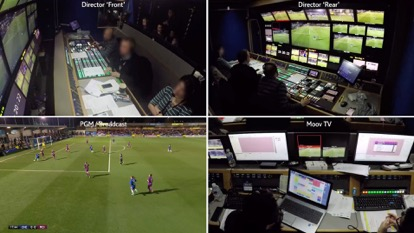
\includegraphics[width=9cm]{Figures/overview.jpg}
    \caption{Ethnographic study at the OB truck of Wembley Stadium (top) and Kingsmeadow Stadium (bottom)}
    \label{fig:overview}
\end{marginfigure}

\keywords{Field study; user interface design; networking; object-based broadcasting; second screens; immersive experiences}

\maketitle

\section{Introduction}

 The world of live-broadcasting is a world of well-defined workflows comprised
 of relatively few but time-critical tasks. The roles inside an Outside-Broadcast
 (OB) truck at a live sporting event are also strictly and subdivided into a few
 discrete stations (Figure~\ref{fig:overview}). Each station has to rely on other
 stations to complete their tasks in a timely manner as to not incur any delays.
 These delays would start to propagate and accumulate down the line and
 potentially affect the transmission of the broadcast. For this reason, it is
 important that any software designed to supplement the workflow in an OB truck
 be easy to use and operate. Moreover, it should facilitate collaboration and
 guarantee timely delivery of the live broadcast.

 This case study presents the development and successful deployment of an
 end-to-end platform for interactive, immersive broadcasts over the Internet at
 a live sport event. In particular, we will detail the requirement gathering phase,
 the aspects of the system used during the broadcast, including \emph{a graphics compositing
 application}, a so-called \emph{Live Triggering} tool for inserting broadcast objects
 into live streams, the camera setup, real-time encoding of video feeds and content
 distribution over the Internet.
 We show the path from a rough first prototype to a complete multi-user platform
 with hardware integration. Finally, we also present a series of trials and
 experiments that were completed along the way, culminating the final
 deployment of the system at the FA Cup final at Wembley stadium in London in
 May 2018. There, the platform was used to support a test-broadcast of the
 football match, delivering the experience to a number of project members in
 their homes.

\begin{marginfigure}
\vspace{-10cm}
\hspace*{-2cm}
    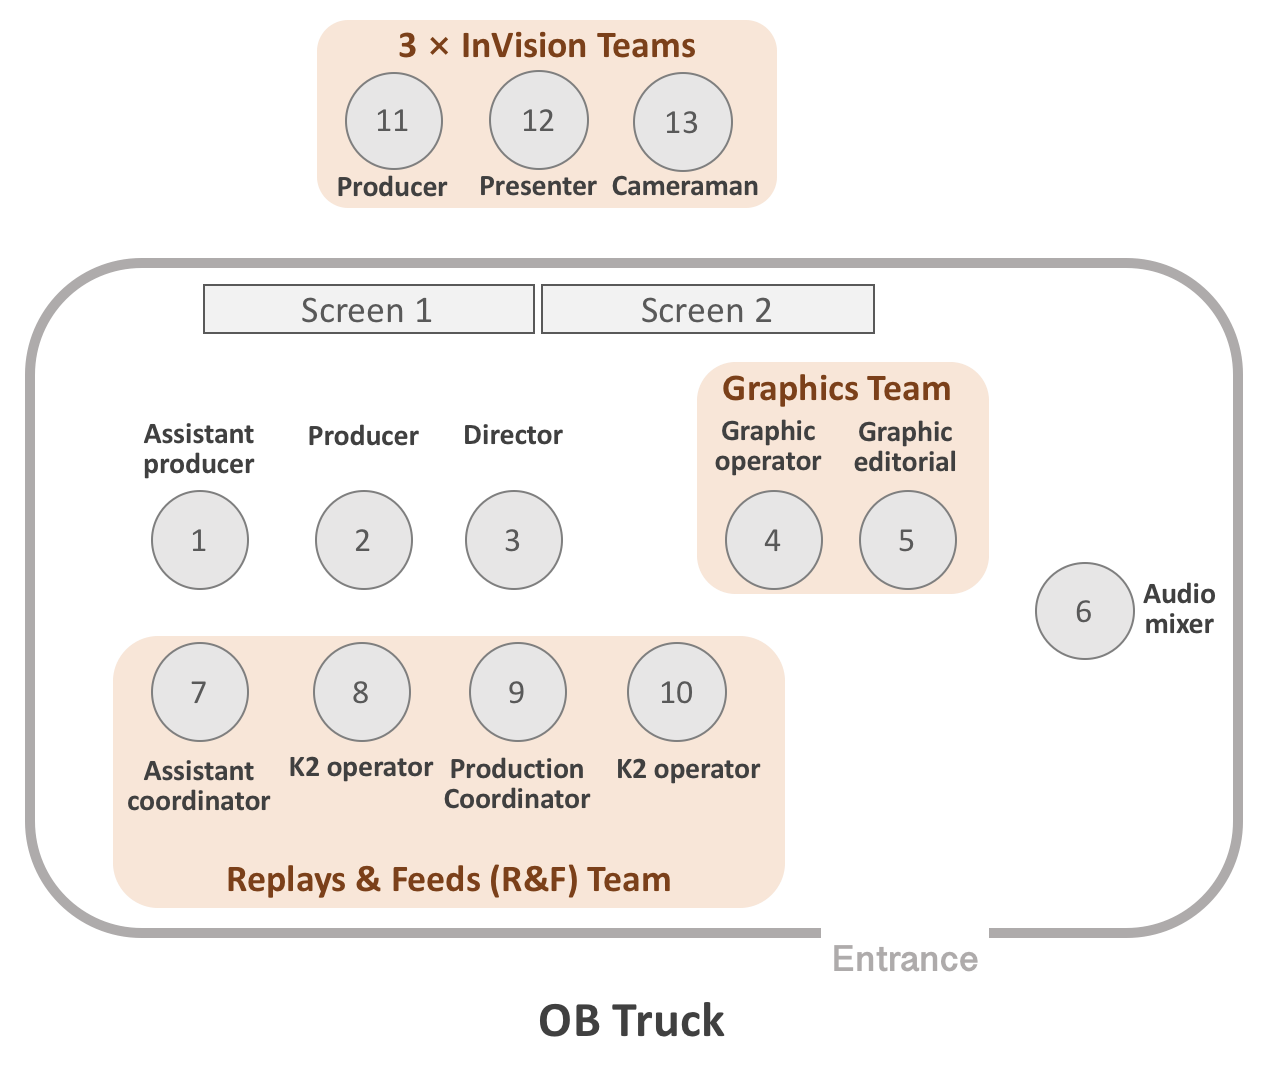
\includegraphics[width=10cm]{Figures/OBtruck.png}
    \caption{Layout of a typical OB truck used at a live sporting event}
    \label{fig:truck}
\end{marginfigure}

At a big sports event such as this, an Outside Broadcasting (OB) truck is the most
common unit for live broadcasting. With its mobility, OB trucks can access any
location and work as a drive-in temporary production control center during live
transmission providing complete video and audio facilities (Figure~\ref{fig:truck}).
An OB truck typically has a wall of monitors shared by all the staff in the truck.
A video production switcher controlled by the director, audio mixer, a team in
charge of recording and playback decks, and a team responsible for live graphics
and so on. It enables the production team to bring the TV audience an authentic
visual representation of an event as it is happening \cite{owens2012, owens2015}.

OB trucks vary in sizes depending on the scale of coverage and the nature of the
event. For a sport event, the coverage includes dozens of stationary cameras, a
couple of handheld cameras, cameras on motorcycles to capture the main athletes
and one or two helicopters with cameras to shoot the \emph{long-shot} of the
scene~\cite{owens2012, Li:2018_TVX}. Today, the production team on OB trucks
orchestrate smoothly to deliver the same linear live program to all kinds TV
screens. The team typically follows a pre-scripted \emph{running order document} that
defines in detail where graphics, visual sources and sound come from and when
they should be \emph{on-air} \cite{Li:2018_TVX}.

As companion screens (e.g. smartphones and tablets) continue to be integrated
into standard television, a challenge the production team facing is to tailor
the content of the TV program so that it works for companion screens as though
it had been uniquely created for them. Content on companion screens are
customizable to enable audience to access additional information next to the TV
screen, and to have interactive and immersive TV viewing
experiences \cite{bentley2017, dowell2015}. However, given the current workload
of the live broadcasting on OB trucks, it is difficult to deliver additional
versions of the program to companion screens. New technologies are required for
this purpose \cite{Li:2018_TVX, armstrong2014}.

\begin{marginfigure}
    % \vspace{1pt}
    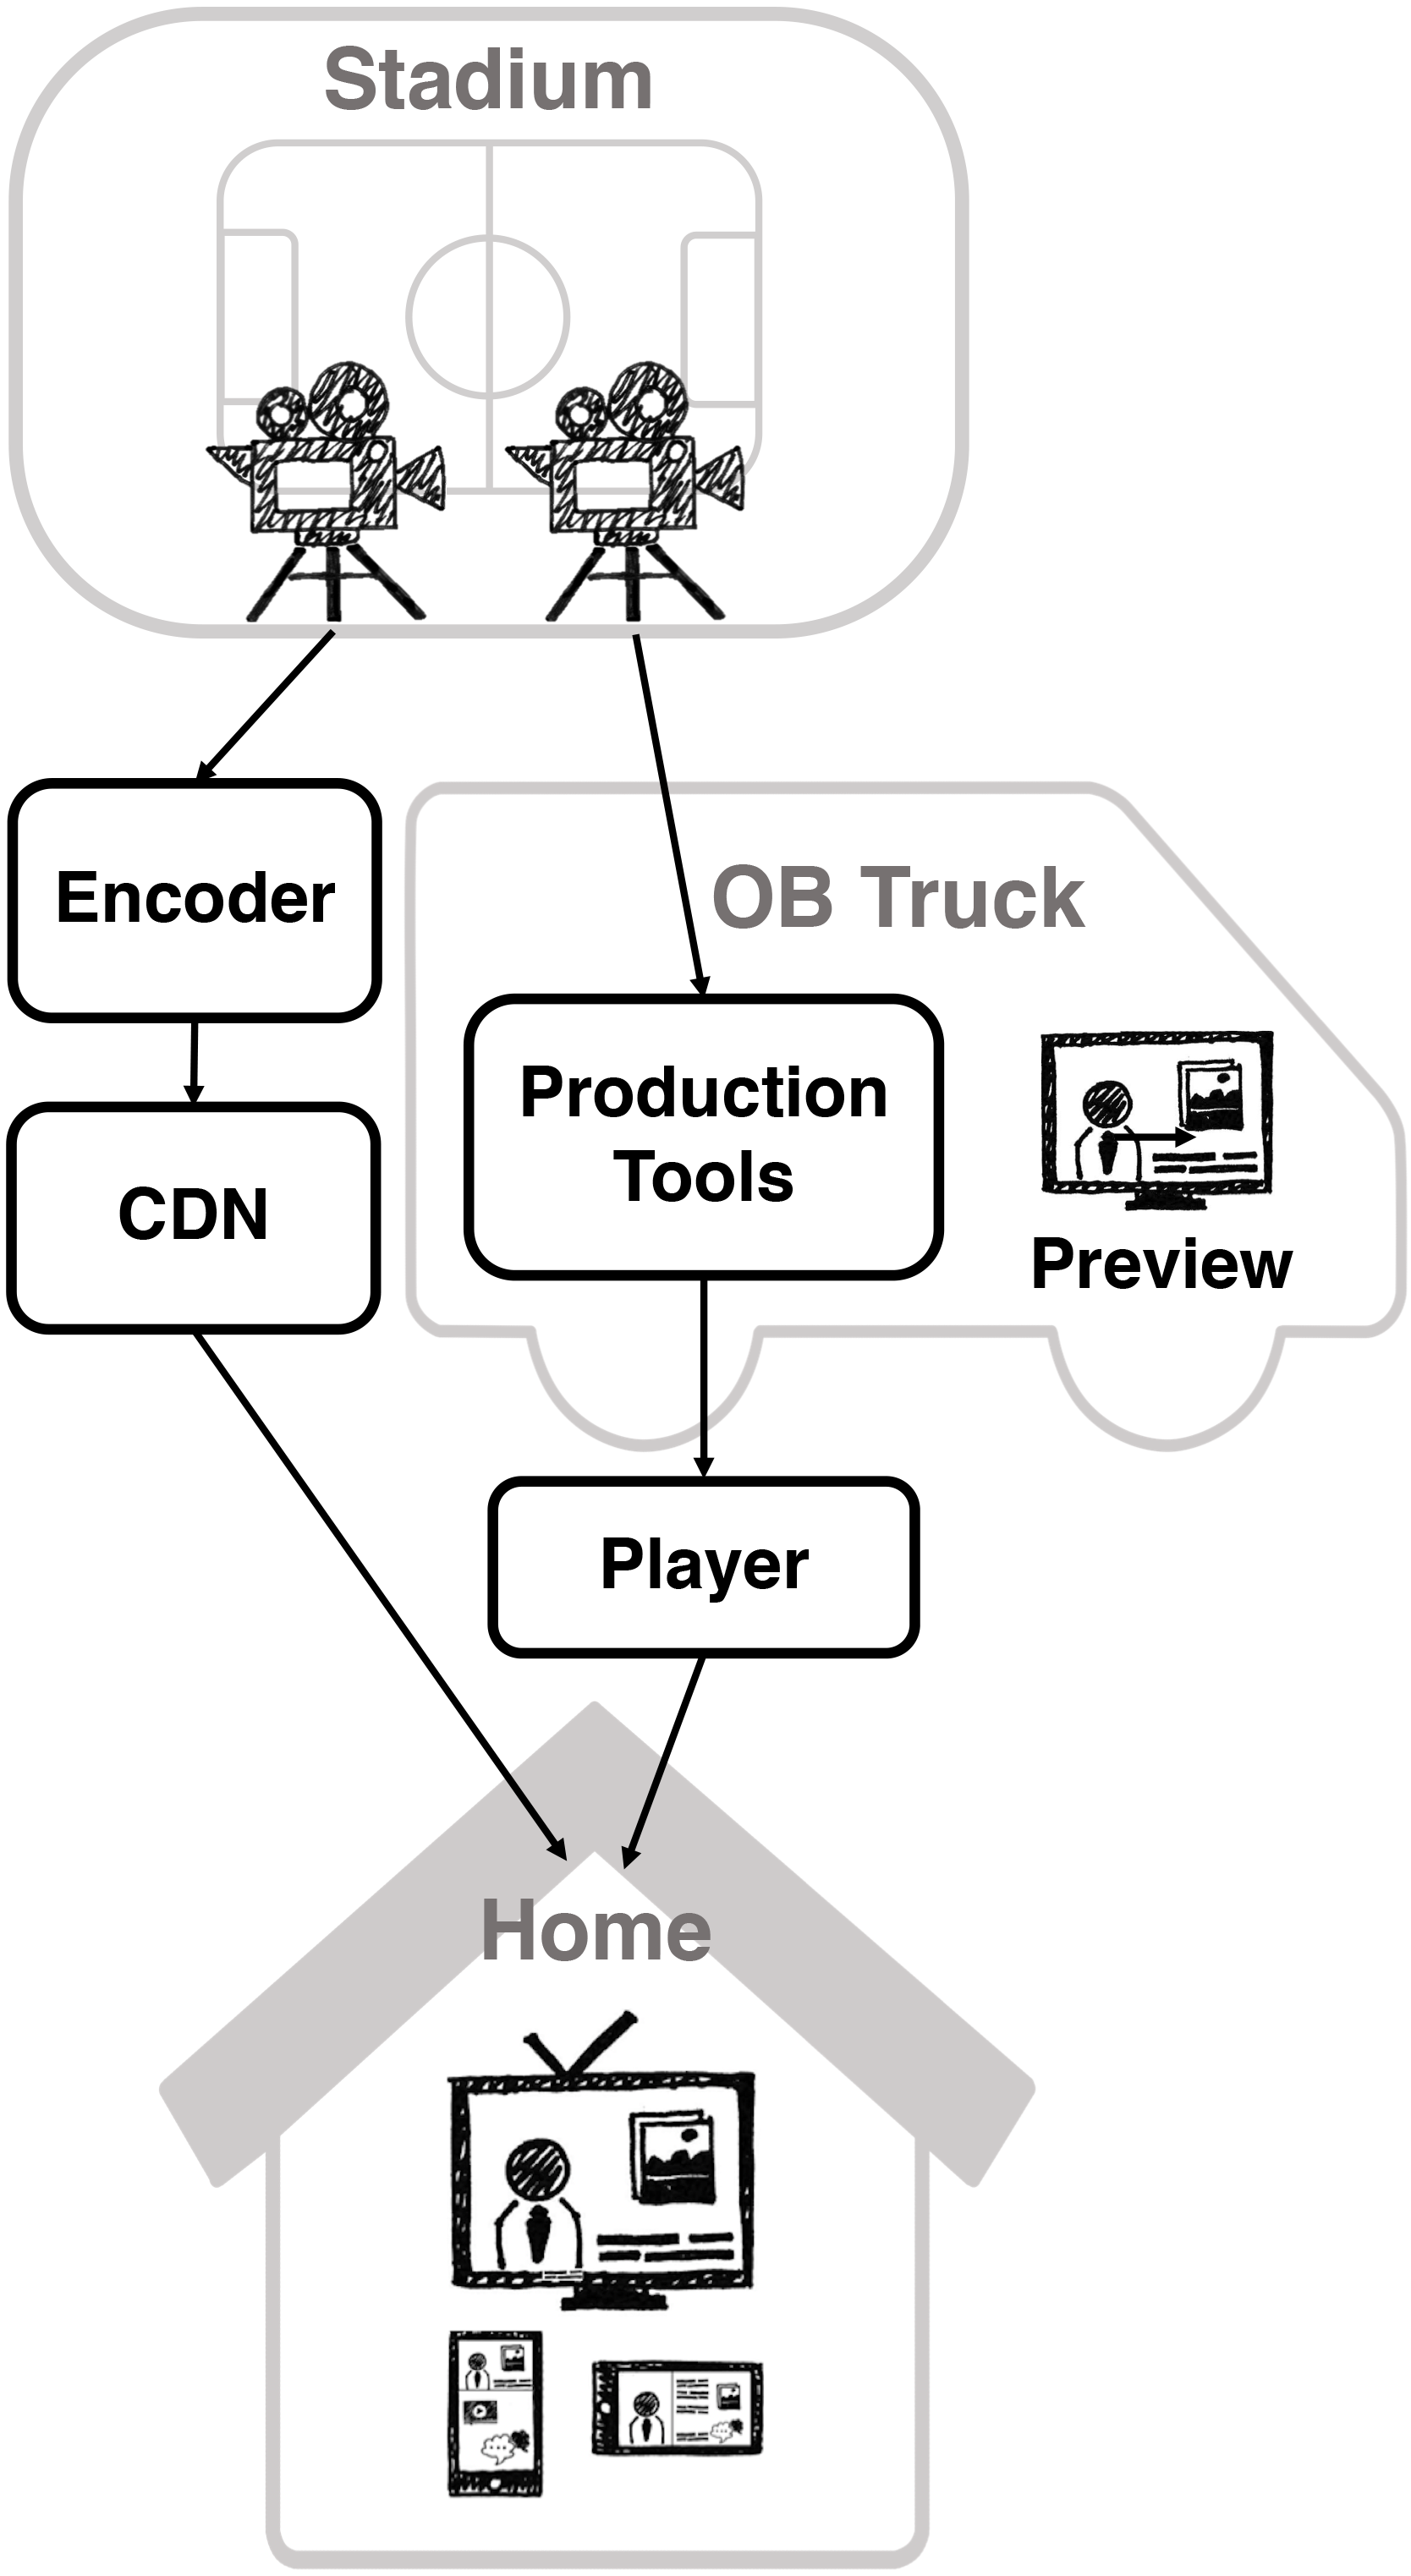
\includegraphics[width=7cm]{Figures/process.png}
    \caption{Production process for a live broadcast with our production platform}
    \label{fig:process}
\end{marginfigure}

One such technology is the \emph{object-based broadcasting} (OBB) approach.
It allows the content of a TV program to
adapt to the requirements of different viewers on multiple companion screens,
without requiring the production team to separately produce different versions
of the program. The \emph{object}, here, refers to different media assets or content
objects that are used to make a TV program \cite{armstrong2014}. The OBB approach
involves breaking down a program into separate objects, typically including
graphics, audio, video, background music, dialogues, subtitles, sound/visual
effects, etc., and including a metadata to describe how these objects can be
assembled on multiple screens. It enables the creation of a flexible, personalized,
and responsive program without increasing the production
workload~\cite{kegel2017, williams2016}. A rough layout of the production process
using our OBB system can be seen in Figure~\ref{fig:process}.

\section{Preparation}
Previously, we have reported successful groundwork for the design and development
of a novel object-based broadcasting platform \cite{kegel2017, Li:2018_CHI, Li:2018_TVX}.
Our next objective was its deployment during a live event like the FA Cup Final
2018 in Wembley. To better understand the challenges of delivering such a trial at
a live football match broadcast, the authors negotiated (via BT Sport) to allow
observation for better understanding of the current workflow involved at an OB
truck. In particular, the following events were observed:

\begin{itemize}
  \item FA Community Shield match at Wembley Stadium on Sunday $6^{th}$ August 2017,
        where access was granted only to one match truck. This event provided us
        with an overview of the director's role in creating the broadcast mix of
        video, graphics and commentary narrative for the match;
  \item Women's Super League match at Kingsmeadow Stadium on Thursday $1^{st}$
        February 2018, where access was granted to observe and record inside the OB
        truck. A number of GoPro cameras were used to capture the pre-broadcast
        preparation and live broadcast activity within the main gallery of the
        truck. These videos were composited into a synchronized quad view video
        along with the broadcast output.
\end{itemize}

The capacity afforded by Wembley Stadium in terms of connectivity,
as well as physical gantry and production space, made it the preferred option as
an event venue. In addition to the more ethnographic observations detailed above,
the research team, working closely with the Chief Engineer and production team
at BT Sport, was allowed to run live tests during two matches at Wembley on $22^{nd}$
April 2018 (FA Cup Semi-Final) and on 12$^{th}$ May 2018 (National League Play-Off Final).

Such observations and tests resulted in a number of requirements, anticipating
operational and technological risks. Such requirements included, for example,
the creation of a number of documents such as the call sheet and the team sheet
(for pre-populating the graphics with the correct player names one hour before
the beginning of the match). The requirements covered as well technological
aspects, such as the pre-production of the assets, the development of the
infrastructure to be deployed at the venue and in the cloud and the access to
various data channels such as the clean video data feeds. Finally, there were
other operational guidelines for, for example, granting access to the researchers
or colocating our mini OB truck in the OB Compound with the other broadcasters.
The following subsections will detail the different preparation steps before the
official match day.

%\subection{Infrastructure}
%A delivery plan was developed in which the first event on 22nd April was used to gain familiarity with the OB facilities at Wembley Stadium and to test live content acquisition and distribution, plus live triggering of production graphics as far as possible while being aware that further development would be required to complete the client experience following this event. The second event, on 12th May, was used as a ‘dress rehearsal’ to test end-to-end system performance and identify remaining issues to be addressed prior to the final event on 19th May for the FA Final Cup. 
%\todo{image about the infrastructure; hopefully from the deliverable; otherwise maybe Jack has one}

\subsection{Graphics}

\begin{marginfigure}
    % \vspace{2cm}
    \hspace*{-2cm}
    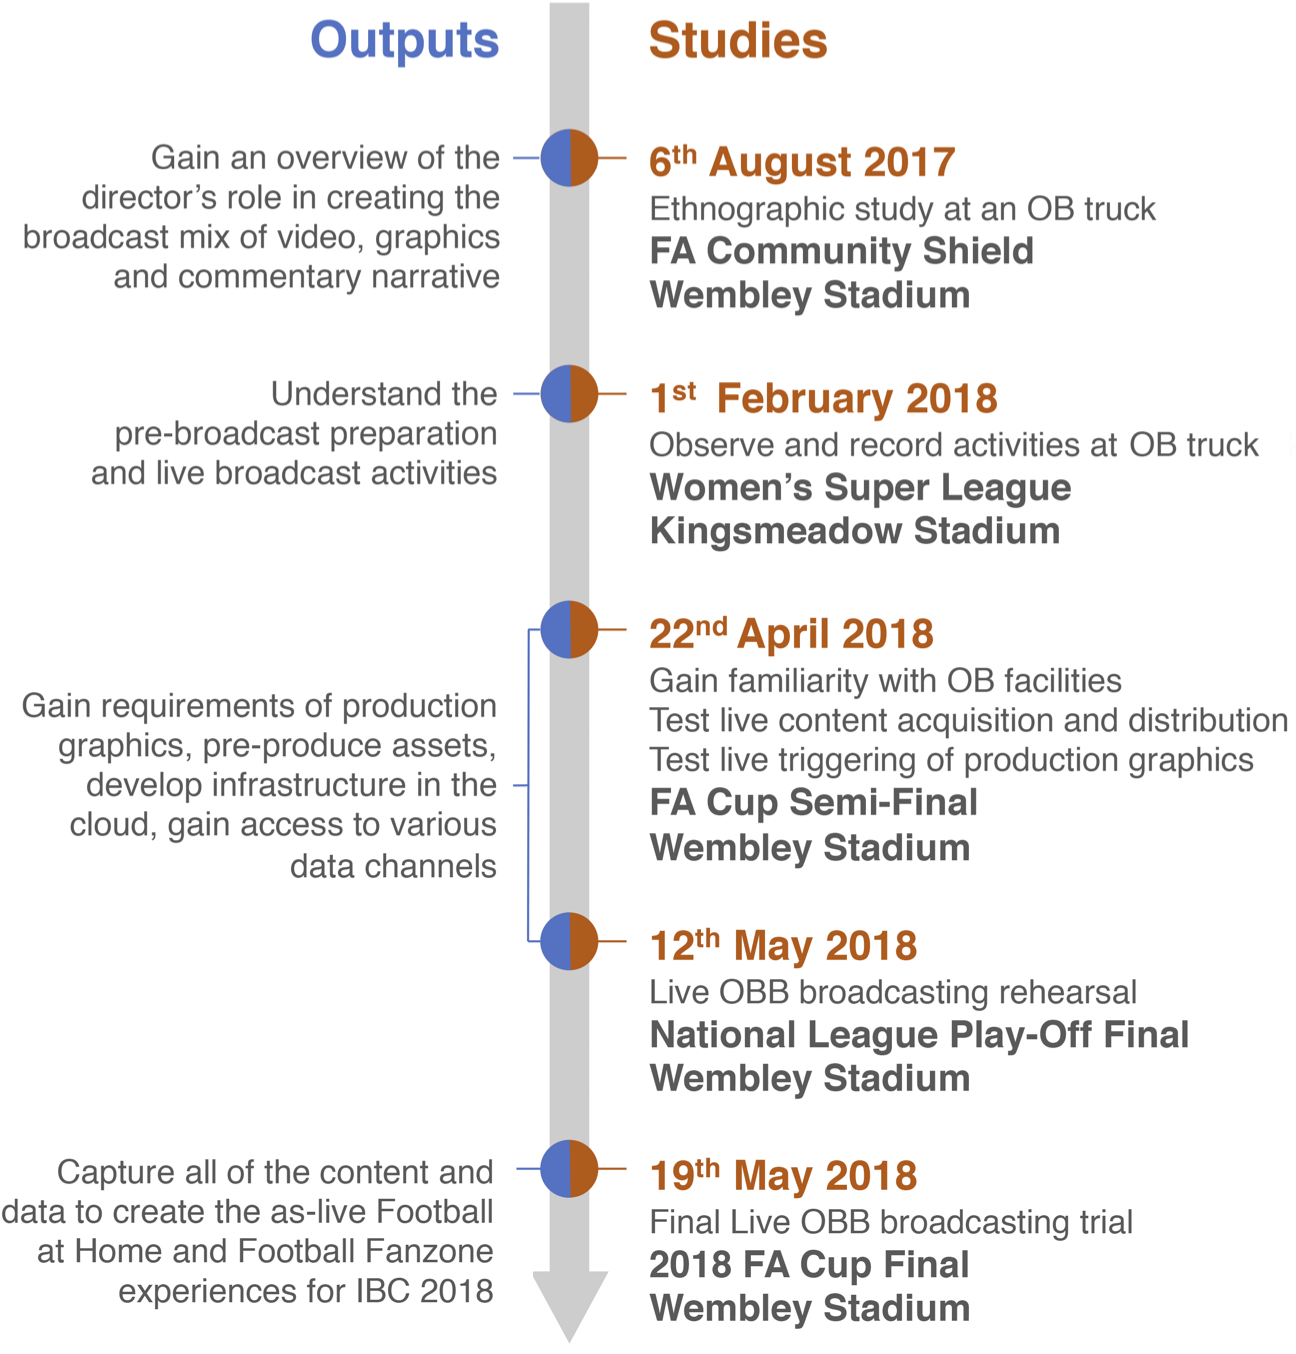
\includegraphics[width=10cm]{Figures/timeline.png}
    \caption{Timeline of the project}
    \label{fig:timeline}
\end{marginfigure}

Object-Based broadcasting provides user-level personalization and it thus
requires all broadcast graphics (non-video visualizations overlaid on top of
the video) to be directly composited on the client device. This is a major shift
from traditional broadcasts, where all graphics are overlaid at the OB Truck,
making the creation process for such graphics quite cumbersome and time consuming.
The design of these graphic elements and animations is thoroughly defined and
specified down to pixel perfection. We tried to adopt a workflow common in traditional
TV stations and networks, which meant that a new purpose-built WYSIWYG design
tool was needed. Since there was no time and resources to create one, the
short-term solution was to adapt an existing one from ChyronHego's product range. The researchers extended the existing
broadcast graphics authoring tool \emph{ChyronHego Prime} with a compatible renderer,
making it usable within our object-based broadcast infrastructure.

\subsection{Production Tool}

Previous work of the research team resulted in a novel model and workflow for
production tools that allow for object-based broadcasting \cite{Li:2018_TVX}.
The tools were intended for covering MotoGP races, but we had the intuition that
they could be adapted for football, and other sports as well. We thus arranged a number
of conversations with professionals working on TV sports broadcast and carefully
observed the recordings from the OB truck at the FA Women's Super League football
game.

\begin{marginfigure}
    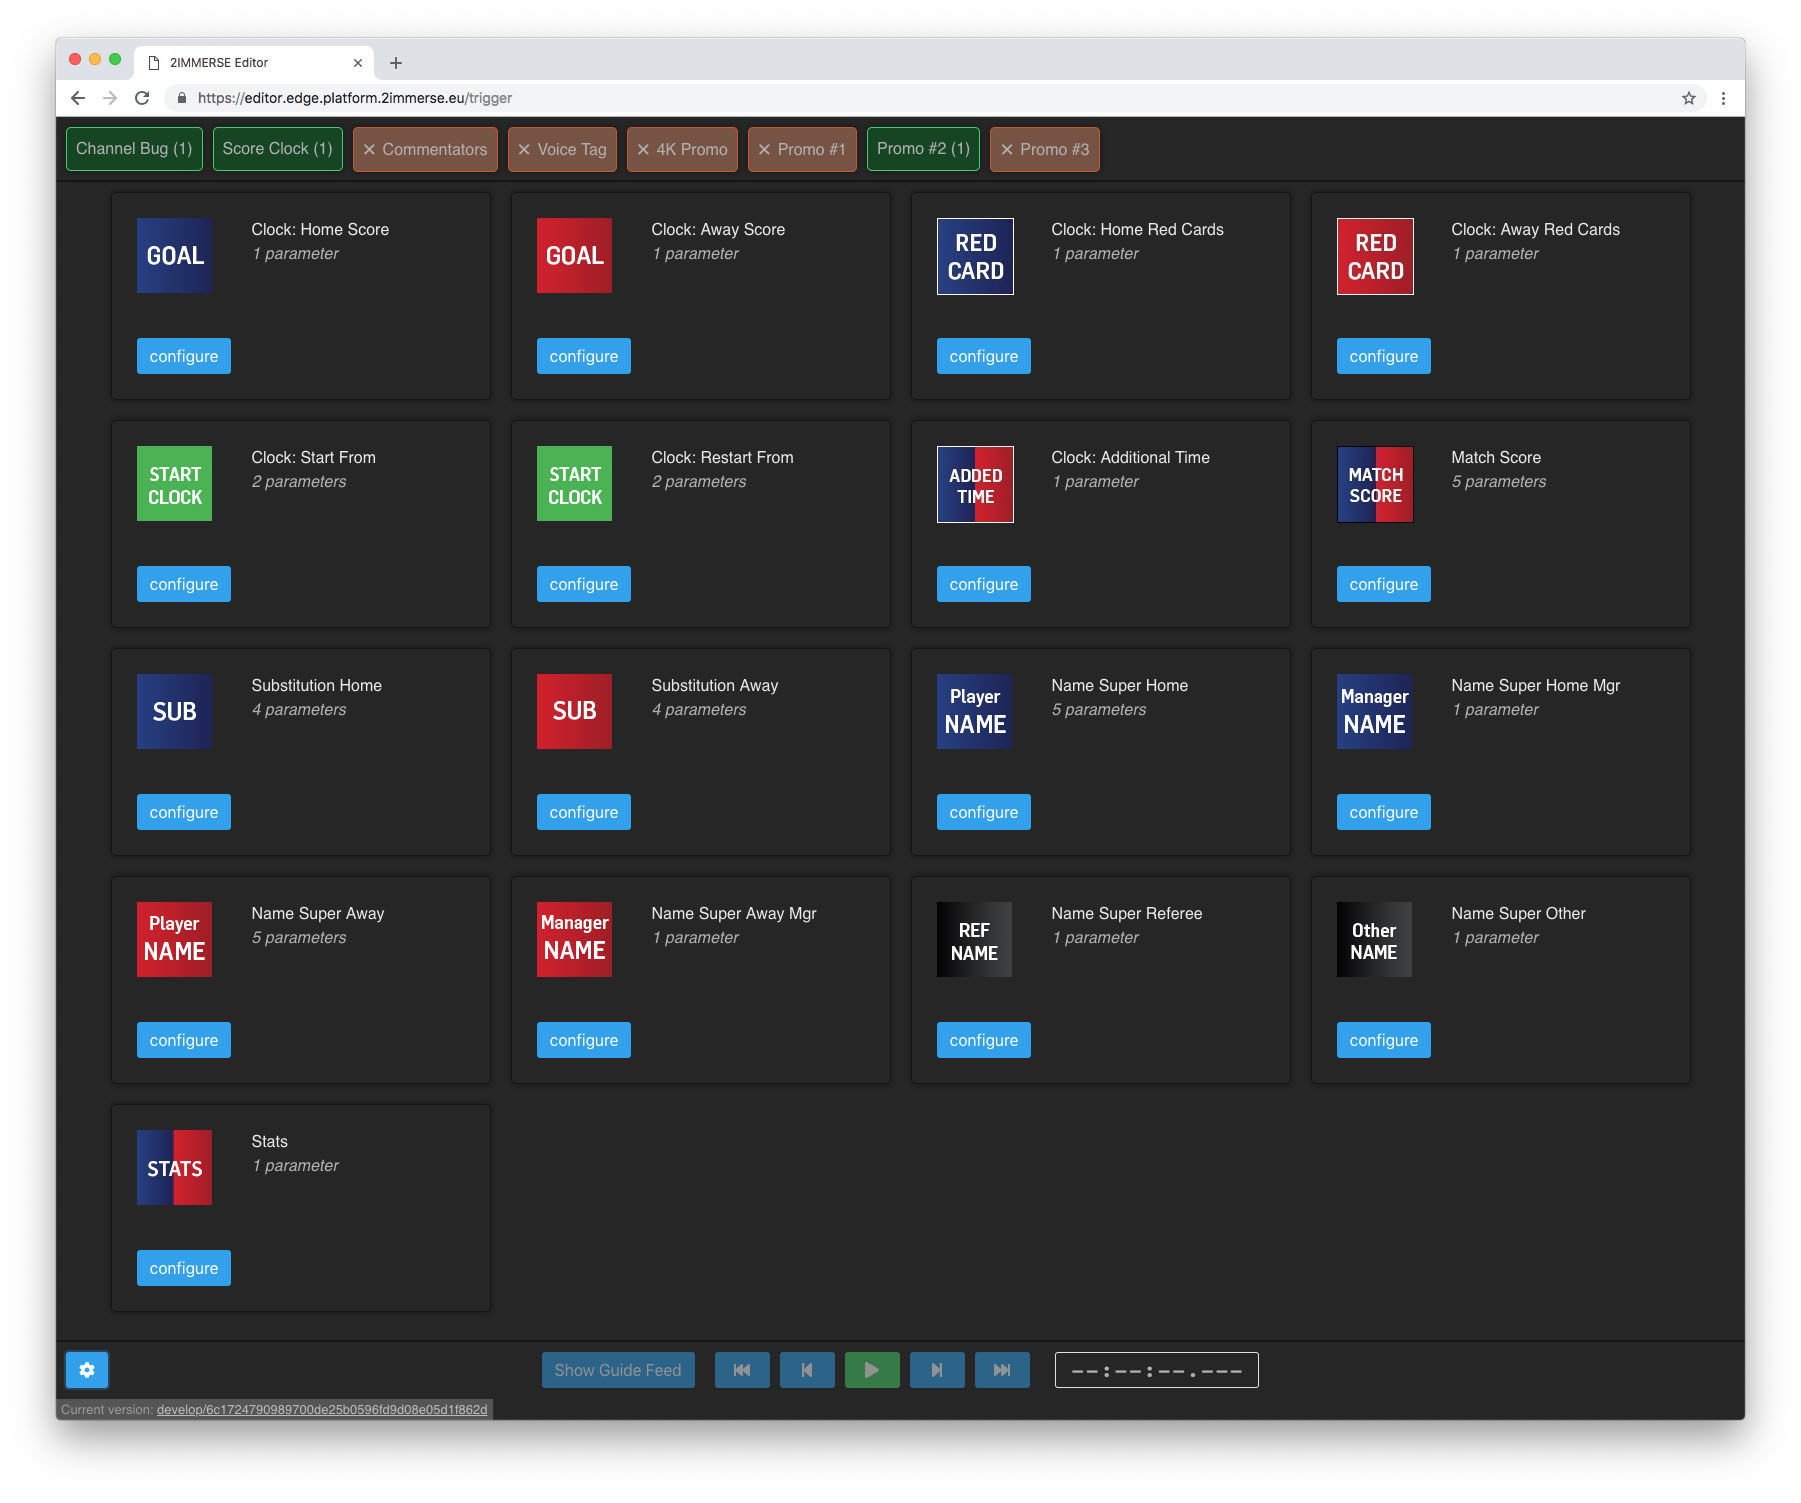
\includegraphics[width=\marginparwidth-10pt]{Figures/triggertool.jpg}
    \caption{Trigger tool (top) and trigger launcher (bottom) in operation}
    \label{fig:triggertool}
\end{marginfigure}

Based on the focus groups and the observations, we concluded that our previous
work was a good starting point, but required some modifications. First, all
controls should be easy to manipulate and to target. Second, the person
preparing the content for, for example, replay clips is not the same one as the
person who decides when and if the content is inserted into the broadcast. The
former task is shared by several people, whereas the latter is usually performed
by either the director or a vision mixer. Finally, we learned that in the truck
there are a lot of special-purpose hardware devices with big buttons and dials,
providing quick access to specific functions.

\begin{marginfigure}
    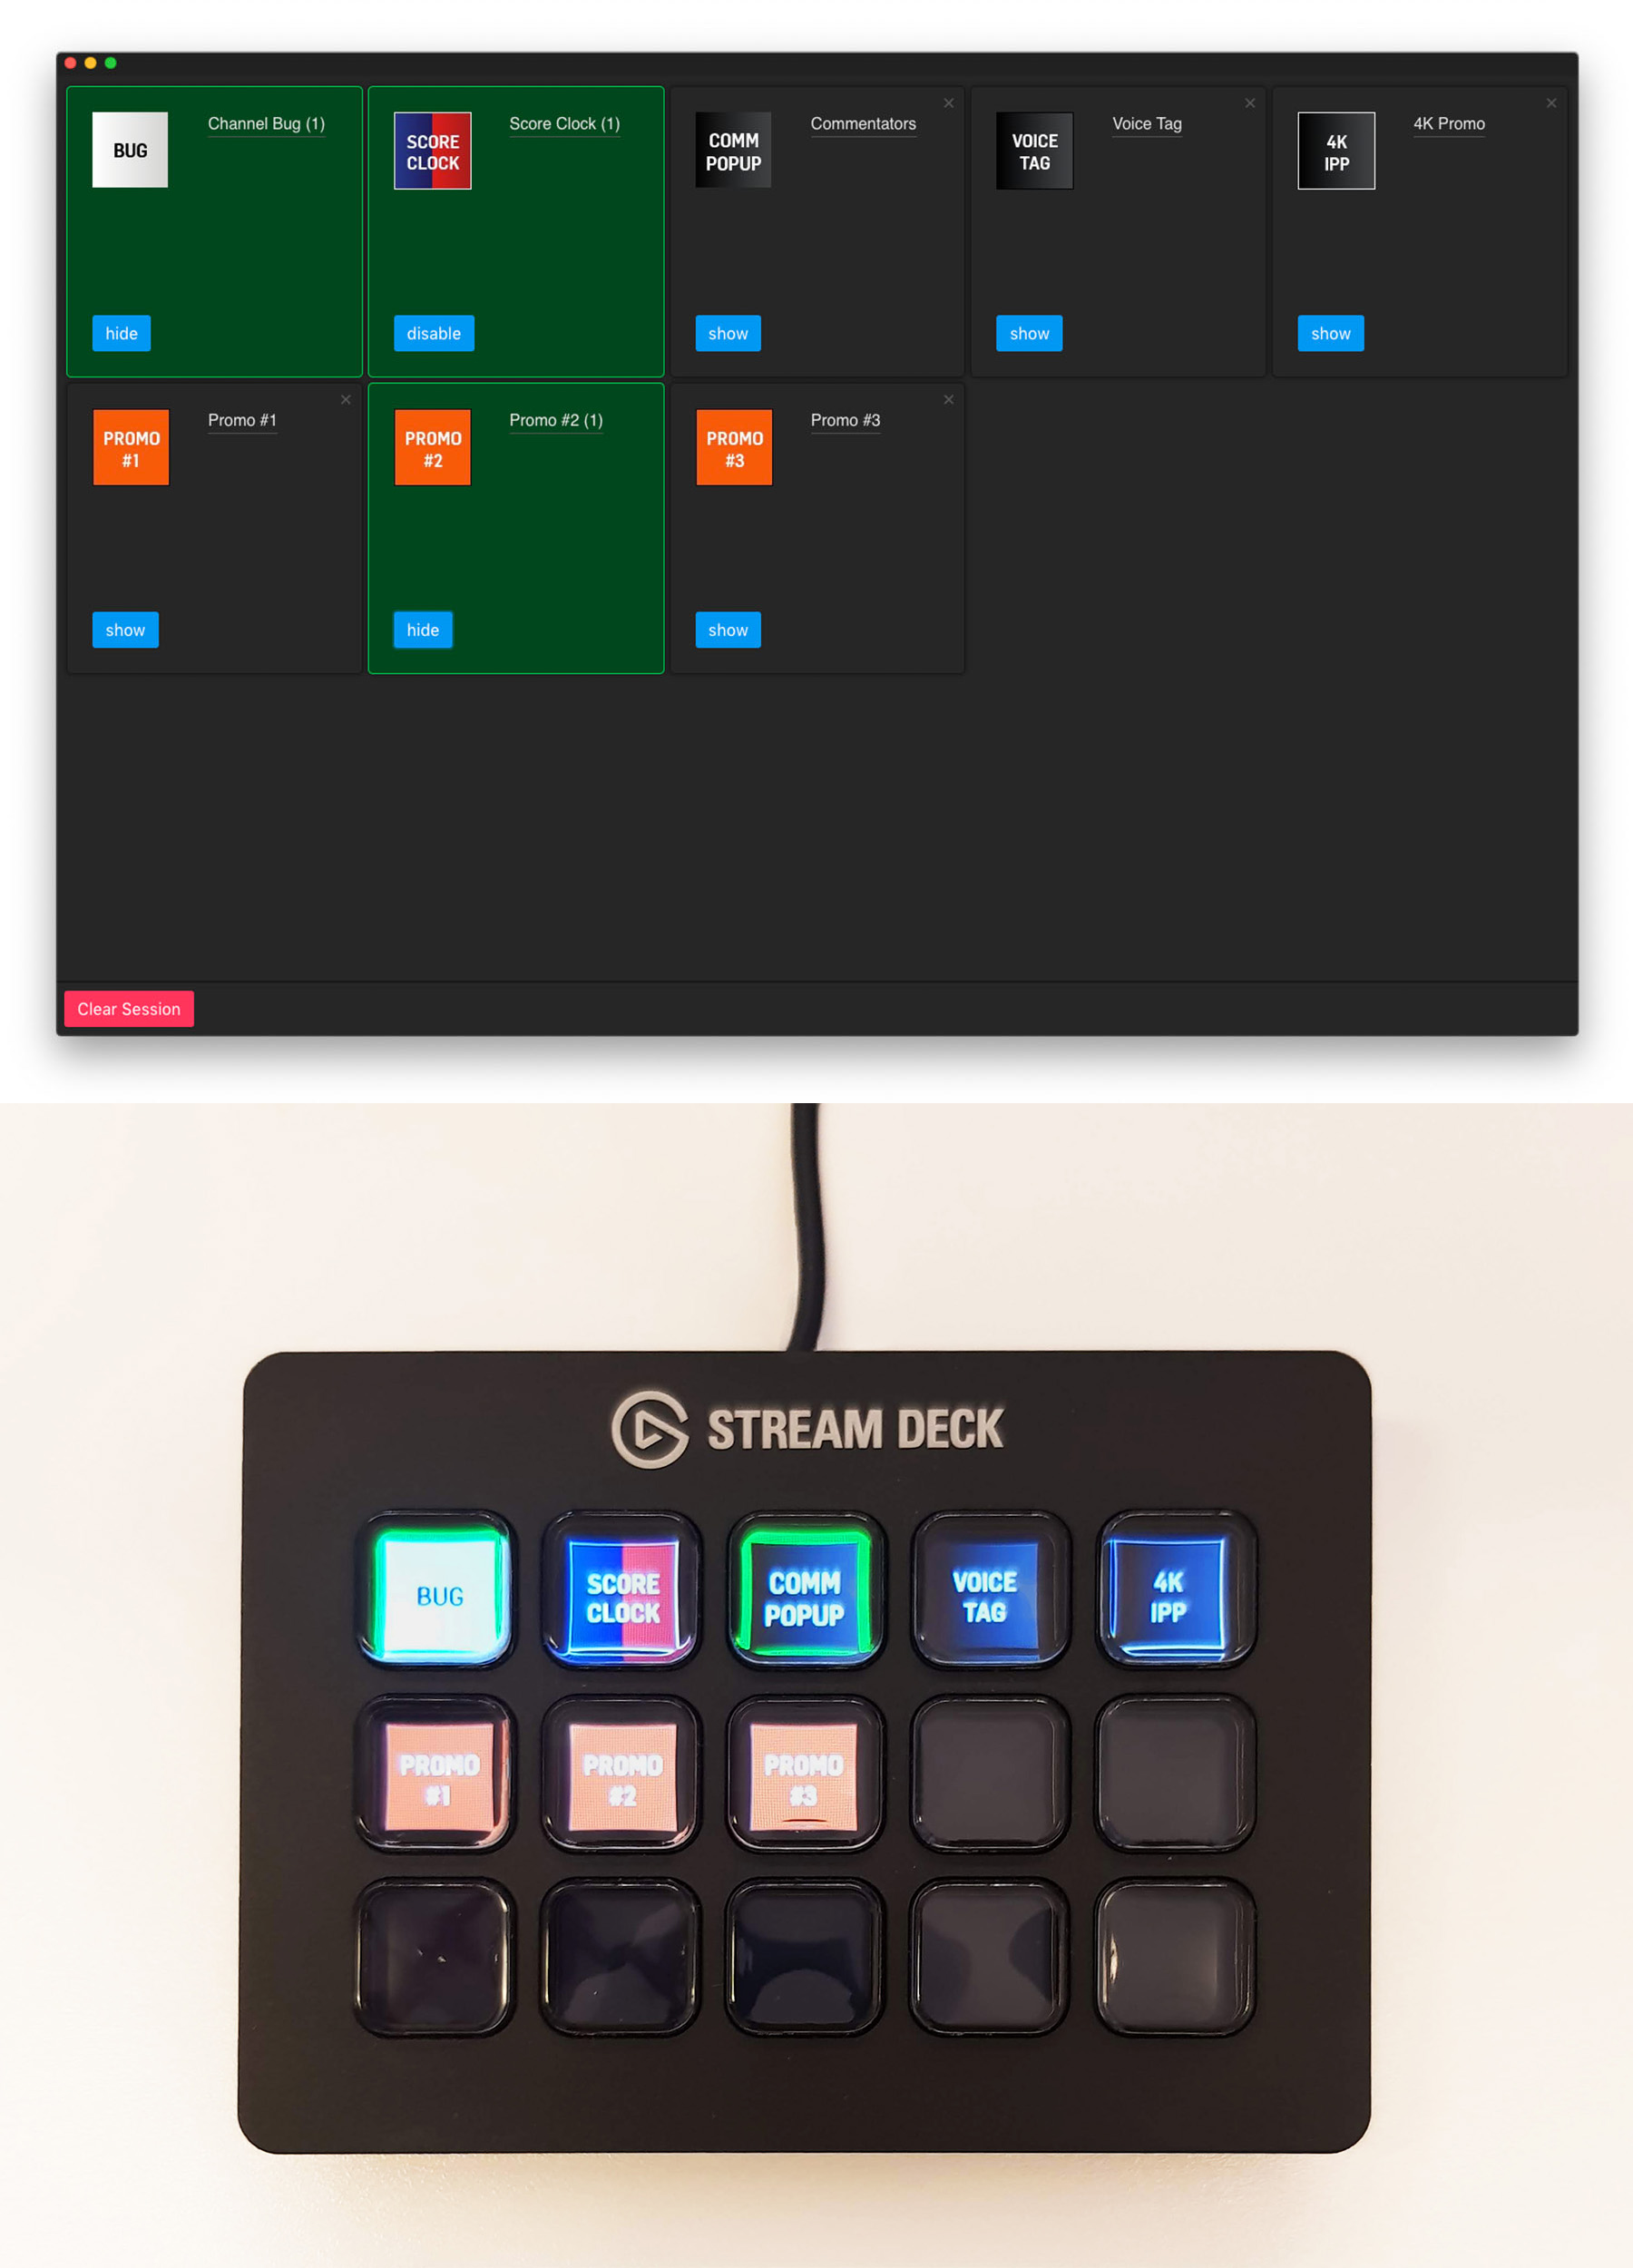
\includegraphics[width=\marginparwidth-10pt]{Figures/streamdeck.jpg}
    \caption{Hardware device \emph{StreamDeck} for operating the trigger launcher}
    \label{fig:streamdeck}
\end{marginfigure}

Based on the new requirements, we designed a new version of our live triggering
tool, diving it into two sub-tasks, each one targeted at a different professional
(Figure~\ref{fig:triggertool}). The first tool, called \emph{Trigger Tool} allows to prepare media
related to the events, such as replay clips or inserting on-screen labels and queueing
them for the director to launch. The second one, called \emph{Trigger Launcher}, intended for the director, can
be used for launching the events when ready, i.e. inserting them into the broadcast.
For the second one, we were able to integrate support for \emph{StreamDeck}, a 
hardware device intended for video-game streamers. The device is equipped with 15
hardware buttons, where each button is backed by a 72x72 pixel LCD screen, plugged into the computer via USB
(Figure~\ref{fig:streamdeck}). This enabled us to map the events rendered in the
trigger launcher application onto the buttons, allowing the user to conveniently launch and
modify events quickly from this console instead of having to use the mouse and
click the corresponding button on the computer screen.

\section{Object-Based Broadcasting during FA Cup Final}
After the preparation work described in the previous section, the research team
was (almost) ready to bring a unique football experience during the FA Cup Final
at Wembley Stadium to people's homes. The football experience was to be a unique, object-based broadcast, since a
multitude of media objects could be assembled in a personalized manner and rendered on
different screens at home: a single primary shared screen (main TV) coupled with
a companion device such as a tablet (Figure~\ref{fig:homeexperience}).

%The main available assets included:
%\textbf{Live Camera Feeds} we broadcast a range of live camera feeds, such as the clean broadcast feeds, the main camera-wide shot, the manager cameras, the team benches, the LH and RH High behind, and the Spider cam.
%\textbf{TV Match GFX}: the BT Sport Match GFX were replicated in terms of style, layout and animations using the modified version of the ChyronHego's Prime authoring tool. These included, among others, the clock, the score, all the players.
%\textbf{Companion Graphics}: the BT Sport design style was adopted when creating the graphics for the companion app GUI. To launch the menu in the companion, the user could tap and access more media about the match (e.g., match overview, match stats, team line ups and replays).

The deployment at Wembley Stadium was centered around our very own OB vehicle, a
Mercedes Sprinter van fitted with two small work areas and basic services
such as power, cable routing, air conditioning and lighting. This vehicle was
essential as a space to safely host and operate the additional components
required for object-based broadcasting. The vehicle was provided by BT Sport
supplier Telegenic, who also provided personnel to support the research team.
The Telegenic team provided essential assistance for gaining access to the
necessary infrastructure and live feeds and provided a listen-only feed of the
Match Director's talkback channel within the vehicle. This enabled the team to
hear and follow the majority of vision and graphics cues given by the director throughout each match and thus
test the object-based production tools in a representative way.
The following paragraphs detail the different components deployed during the day
of the match.

\vspace{5pt}\noindent\textbf{Live Camera Feeds.} The project team requested access to a range of live
camera feeds. We had access to the clean and dirty (Match Director's output)
broadcast feeds, the main camera-wide shot, the manager cameras, the team
benches, the LH and RH High behind, and the Spider cam. Each camera feed was
provided in HD-SDI format in a separate coaxial cable routed from the BT Sport
production truck to the vehicle.

\begin{marginfigure}
\hspace*{-0.5cm}
    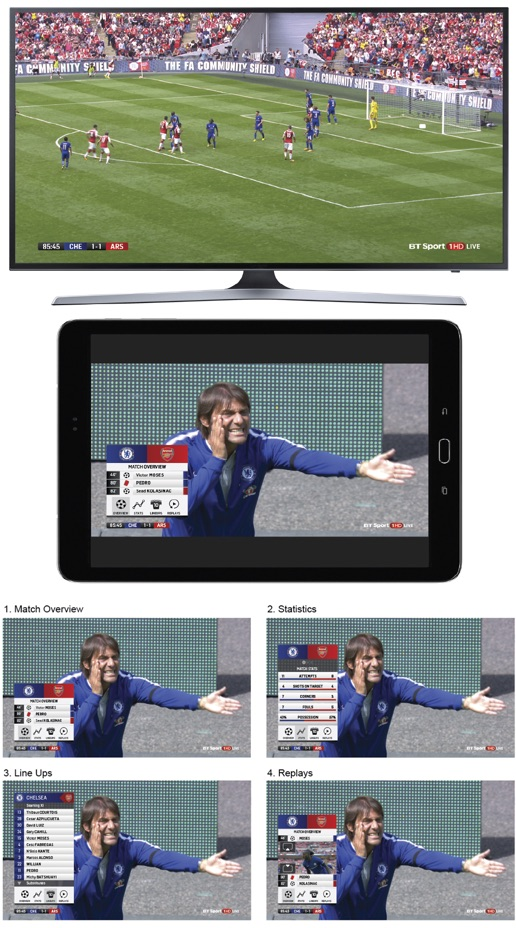
\includegraphics[width=7cm]{Figures/footballathome1.jpg}
    
    \caption{Experience at home as viewed by an end user: television screen (top), tablet (middle) and user-customizable screen configurations for companion screen (bottom)}
    \label{fig:homeexperience}
\end{marginfigure}

\vspace{5pt}\noindent\textbf{Live Encoding.} Two live streaming encoders were loaned for the duration
of the tests by BT supplier AWS Elemental, who also provided technical assistance
with configuring them and resolving issues. Each encoder was capable of live
encoding a multi-layer DASH representation of 8 HD-SDI input streams. Once
encoded, the DASH segments were uploaded to the CDN Origin Server, from where
they could be consumed by the client applications. Given that the FA Cup Final
match was simultaneously broadcast free-to-air in the UK, it was agreed that
stream encryption need not be used, but instead access control was applied to
the Origin Server so that client apps were required to authenticate before they
could download the stream.

\vspace{5pt}\noindent\textbf{Internt Uplink.} The use of additional live encoders also necessitated
the provision of Internet uplink capacity dedicated to the OB vehicle. This
proved to be the most challenging dependency. In order to upload the 3-layer
MPEG-DASH representation for 8 distinct live streams, while providing headroom
for audio streams and signaling, at least 100Mbps upstream was required. In the
end, a dedicated BT uplink was used.

\vspace{5pt}\noindent\textbf{Triggering Interface.} One half of the OB vehicle was dedicated to live
triggering of object-based production graphics using the production tools
described above. The tools ran on a laptop PC with the addition of an Elgato
Streamdeck programmable keypad. the production tools communicate with our
platform services, which were hosted off-site within an Amazon Web Services
environment. The production tools were modified as well to enable the preview
client to display the live feed from the capture device within the primary video
player component, rather than opening the delayed MPEG-DASH stream from the CDN
Origin Server.

\vspace{5pt}\noindent\textbf{Virtual Placement.} The Virtual Placement system was set up independently
of the live production tools in one half of the vehicle during the FA Cup Final
event. Its purpose was to enable the ChyronHego team to test their new workflow,
enabling object-based virtual graphics to be rendered in a personalised way on
a viewer's client device. This workflow uses ChyronHego's player tracking
technology, \emph{Tracab}, based on dedicated networked cameras installed in a stadium
to determine the location of players on the pitch at any point in time. Virtual
Placement, at the same time, uses calibration parameters derived from a wide-angle
camera to enable graphics to be rendered on the live broadcast feed as if they
were part of the three-dimensional scene. By synchronizing Tracab player tracking
data with Virtual Placement camera tracking data and streaming it to a client
device, it should be possible for the client device to render virtual graphics
around players as they move across the pitch - for example to provide additional
statistics or a comparison between a viewer's favourite players.

\vspace{5pt}\noindent\textbf{Content Distribution Network (CDN).} The 2-IMMERSE platform \cite{kegel2017} was the most significant
off-site components, playing a vital role in the delivery of the end-to-end live
tests. As with all 2-IMMERSE Distributed Media Applications, the Layout and
Timeline services were responsible for orchestrating the viewer experience on
the TV and companion devices. In addition, for these tests it was also necessary
to orchestrate the Live Preview Client. Another crucial extension to the platform
was the ability for timeline updates which were created by the Live Triggering
Tool to be automatically inserted by the Editor service within the active
timelines of every client context which was watching the match, while accounting
for the fact that off-site viewers' timelines would be delayed by up to a minute
due to large buffers resulting from the MPEG-DASH live streaming configuration.

%\textbf{Replay} During some live events, the on-site BT Sport production team create replays that are automatically uploaded to the EVS C-Cast platform  for on-demand viewing and distribution to existing mobile applications. In order to provide interactive access to replays on demand within the 2-IMMERSE Football client applications, it was necessary to create an additional off-site workflow in which the required replays were extracted from C-Cast, converted to the MPEG-DASH adaptive bitrate streaming format, and made available on the 2-IMMERSE CDN Origin Server. The project team configured an instance of cloud-based AWS Elemental MediaConvert to automatically encode replay files into a suitable MPEG-DASH format when uploaded to a specific Amazon S3 location. The encoded output is then automatically transferred to the 2-IMMERSE Origin Server, while at the same time the necessary metadata describing the reply is created so that the appropriate menus within the client applications can be updated to provide access to the replay.

\section{Discussion}
%  \todo{to include some photo from IBC}
%  \todo{include a paragraph about IBC as a successful outcome of Wembley}
%  \todo{to discuss about the impact of the work on BT Sports, as a showcase of future valuable technology}
%  \todo{to discuss about the new toolset developed by Chyron Hego for creating GFX and distribute them in an object-based oriented manner}
%  \todo{to discuss about our production tools and the next steps}
%  \todo{to bring back other papers and experiences, like the one from Frank Bentley}

\begin{marginfigure}
    \vspace{-18pc}
    \hspace*{-1cm}
    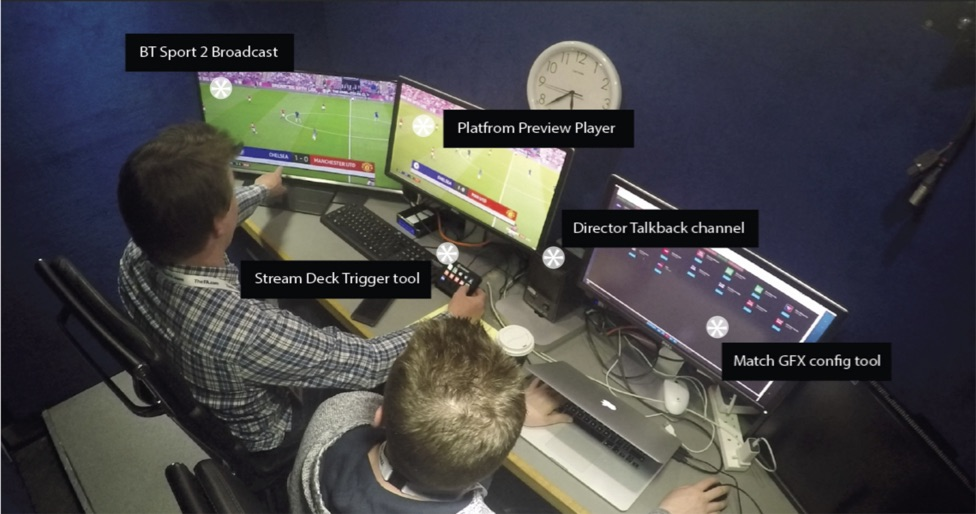
\includegraphics[width=8cm]{Figures/liveproduction.jpg}
    \caption{The setup of the system in the OB truck at the stadium}
    \label{fig:liveproduction}
\end{marginfigure}

\begin{marginfigure}
    \hspace*{-1cm}
    \includegraphics[width=8cm]{Figures/IBC.jpg}
    \caption{Presenting the project at IBC 2018 in Amsterdam}
    \label{fig:ibc}
\end{marginfigure}

\textbf{New challenges for the industry.} Over the course of the project (Figure~\ref{fig:timeline}), we successfully bridged the gap between lab research 
and the key players in the production chain (e.g. BT Sports, MoovTV),
motivating them to think of developing use cases or tools taking advantage of OBB. As noted by Bentley et.al.~\cite{bentley2009},
the ethnographic-style field study can take new concepts to real users in
early stages of development, quickly illuminating potential
bottlenecks and challenges. In our trial, the first challenge was to smooth the
graphics creation workflow in this time-critical environment. To
do so, we used an existing authoring tool (ChyronHego Prime) with a graphical
interface but an XML-based storage format, enabling a \textit{designer} to create
graphics without needing a \textit{developer}. However, the application was not specifically designed for OBB processes. New production tools to visually create OBB assets are needed. The second challenge addressed is the usability of the OBB production tools. A refinement of our tools towards re-usability of content and customization of graphics can be expected. 

\vspace{5pt}\noindent\textbf{Impact on the industry.} Based on the video assets
collected from the Wembley trial (Figure~\ref{fig:liveproduction}), the project team developed a more complete and
polished as-live multiscreen FA Cup demonstration, showing how production
tools were used to edit and broadcast graphics in an OBB manner. Together with
the production tools, it exhibited how viewers can personalize their experiences
through companion screens in the context of the home. The
demonstration was successfully presented at the \emph{Future Zone} of IBC (Figure~\ref{fig:ibc}), the world's
most influential media technology exhibition. The exhibition received a wide
range of audience including key stakeholders from the broadcast industry,
university researchers, production teams. All of them believed "OBB is the future".

\section{Future Work \& Conclusion}

To help integrate the OBB approach into the existing
production workflow, the next step is to develop a pre-production tool with a
graphical interface, to allow people without programming skills to author
multiscreen TV content. The preproduction tool aims at reducing the workload of
the live broadcasting by creating a hierarchical overview of the content and
arranging media objects on a storyline ahead of time \cite{Li:2018_TVX}. The
prototype of the pre-production tool is expected to be tested by a group of
producers and directors in the end of November, 2018. The live trial at Wembley Stadium for the 2018 FA Cup Final was a
milestone to help the OBB approach to make an impact. Through observing two live football matches, the
content acquisition and distribution was tested and the live production tools
were refined to be able to trigger all match graphics during the match.
Our objective of authoring a live end-to-end OBB experience and testing the
reach and scalability of our solution was achieved.

\bibliography{sample-bibliography-sigchi-a}
\bibliographystyle{ACM-Reference-Format}

\end{document}
